\section{Model Evaluation and Selection}\label{class:evaluation}

\begin{frame}{Model Evaluation and Selection}
	\begin{itemize}
		\item \textbf{Evaluation metrics:}
		      \begin{itemize}
			      \item How can we measure accuracy?
			      \item Other metrics to consider?
		      \end{itemize}
		\item \textbf{Use {\color{airforceblue}test} set of class-labeled tuples instead of training set when assessing accuracy.}
		\item \textbf{Methods for estimating a classifier's accuracy:}
		      \begin{itemize}
			      \item Holdout method, random subsampling.
			      \item Cross-validation.
			      \item Bootstrap.
		      \end{itemize}
		\item \textbf{Comparing classifiers:}
		      \begin{itemize}
			      \item Confidence intervals.
			      \item Cost-benefit analysis and ROC curves.
		      \end{itemize}
	\end{itemize}
\end{frame}

\begin{frame}{Confusion Matrix and Evaluation Metrics}
	Given $M$ classes, an entry $C^{(m)}_{ij}$ in an $M \times M$ confusion matrix
	indicates the number of tuples in class $i$ that were labeled by the
	classifier as class $j$.
	\begin{columns}[T]
	\begin{column}[T]{0.45\textwidth}
		\begin{tabular}{c|c|p{1cm}|p{1cm}|c|}

			\multicolumn{2}{c|}{\multirow{2}{*}{}} & \multicolumn{2}{c|}{Predicted Class} &                                           \\\cline{3-4}
			\multicolumn{2}{c|}{}                  & $C_1$                                & $\neg C_1$  & Total                       \\\hline
			\multirow{2}{*}{True Class}            & $C_1$                                & \textbf{TP} & \textbf{FN}    & \textbf{P} \\\cline{2-4}
			                                       & $\neg C_1$                           & \textbf{FP} & \textbf{TN}    & \textbf{N} \\\hline
			\multicolumn{2}{r|}{Total}             & \textbf{P'}                          & \textbf{N'} & \textbf{P + N}
		\end{tabular}

	\end{column}

	\begin{column}[T]{0.5\textwidth}
		\footnotesize
		\begin{itemize}
			\item \textbf{True Positives} = correctly classified tuples.
			\item \textbf{True Negatives} = correctly classified tuples.
			\item \textbf{False Positives} = negative tuples incorrectly classified as positive.
			\item \textbf{False Negatives} = positive tuples incorrectly classified as negative.
		\end{itemize}
	\end{column}
\end{columns}


	\textbf{Accuracy:}
	\vspace*{-1em}
	\begin{columns}
		\begin{column}{0.55\textwidth}
			\begin{itemize}
				\item Percentage of correctly classified tuples.
				\item Also known as the (overall) recognition rate.
				\item Most effective with a \textit{balanced dataset}.
				\item Inverse: \textbf{Error rate} as the misclassification rate.
			\end{itemize}
		\end{column}
		\begin{column}{0.4\textwidth}
			\vspace*{-1.2em}
			\begin{align}
				\text{Accuracy}   & = \frac{\text{TP} + \text{TN}}{\text{P} +  \text{N}} \\
				\text{Error Rate} & = 1 - \text{Accuracy}                                \\
				                  & = \frac{\text{FP} + \text{FN}}{\text{P} + \text{N}}
			\end{align}
		\end{column}
	\end{columns}
\end{frame}

\begin{frame}{Confusion Matrix and Evaluation Metrics (II)}
	\begin{columns}[T]
	\begin{column}[T]{0.45\textwidth}
		\begin{tabular}{c|c|p{1cm}|p{1cm}|c|}

			\multicolumn{2}{c|}{\multirow{2}{*}{}} & \multicolumn{2}{c|}{Predicted Class} &                                           \\\cline{3-4}
			\multicolumn{2}{c|}{}                  & $C_1$                                & $\neg C_1$  & Total                       \\\hline
			\multirow{2}{*}{True Class}            & $C_1$                                & \textbf{TP} & \textbf{FN}    & \textbf{P} \\\cline{2-4}
			                                       & $\neg C_1$                           & \textbf{FP} & \textbf{TN}    & \textbf{N} \\\hline
			\multicolumn{2}{r|}{Total}             & \textbf{P'}                          & \textbf{N'} & \textbf{P + N}
		\end{tabular}

	\end{column}

	\begin{column}[T]{0.5\textwidth}
		\footnotesize
		\begin{itemize}
			\item \textbf{True Positives} = correctly classified tuples.
			\item \textbf{True Negatives} = correctly classified tuples.
			\item \textbf{False Positives} = negative tuples incorrectly classified as positive.
			\item \textbf{False Negatives} = positive tuples incorrectly classified as negative.
		\end{itemize}
	\end{column}
\end{columns}

	\begin{columns}
		\begin{column}{0.4\textwidth}
			\begin{itemize}
				\item \textbf{Sensitivity} = True positive rate.
				\item \textbf{Specificity} = True negative rate.
				\item \textbf{Precision} = Measure of exactness.
				\item \textbf{Recall} = Measure of completeness.\\
				      Perfect score is 1.0.\\
				      Inverse relationship with precision.
			\end{itemize}
		\end{column}

		\begin{column}{0.6\textwidth}
			\begin{align}
				\text{Sensitivity} & = \frac{\text{TP}}{\text{P}}              & = \frac{\text{TP}}{\text{TP} + \text{FN}} & = \text{Recall} \\
				\text{Specificity} & = \frac{\text{TN}}{\text{N}}                                                                            \\
				\text{Precision}   & = \frac{\text{TP}}{\text{TP} + \text{FP}}
			\end{align}
		\end{column}
	\end{columns}
\end{frame}

\begin{frame}{Confusion Matrix and Evaluation Metrics (III)}
	\textbf{F-Measure}: Combines precision and recall in one single measure.

	\begin{columns}
		\begin{column}{0.5\textwidth}
			\begin{center}
				\textbf{$\text{\textbf{F}}_1$ Measure}
			\end{center}
			\begin{align}
				\text{F}_1 = \frac{2 \times \text{Precision} \times \text{Recall}}{\text{Precision} + \text{Recall}}
			\end{align}

			\begin{itemize}
				\item Harmonic mean between precision and recall.
				\item Equal weight to both measures.
			\end{itemize}
		\end{column}

		\begin{column}{0.5\textwidth}
			\begin{center}
				\textbf{$\text{\textbf{F}}_\beta$ Measure}
			\end{center}
			\vspace*{-.5em}
			\begin{align}
				\text{F}_\beta = \frac{(1 + \beta^2) \times \text{Precision} \times \text{Recall}}{\beta^2 \times \text{Precision} + \text{Recall}}
			\end{align}

			\begin{itemize}
				\item Weighted measure.
				\item Gives $\beta$-times more weight to precision.
			\end{itemize}
		\end{column}
	\end{columns}
\end{frame}

% TODO: Update example with confusion matrix
\begin{frame}{Example: Confusion Matrix and Evaluation Metrics (I)}
	\begin{tabular}{|c|c|c|c|}
		\hline
		Actual class/predicted class: & buys\_computer = yes & buys\_computer = no & Total \\\hline
		buys\_computer = yes          & \textbf{6954}        & \textbf{46}         & 7000  \\\hline
		buys\_computer = no           & \textbf{412}         & \textbf{2588}       & 3000  \\\hline
		Total                         & 7366                 & 2634                & 10000 \\\hline
	\end{tabular}
\end{frame}


\begin{frame}{Example: Confusion Matrix and Evaluation Metrics (II)}
	\centering
	\begin{tabular}{|c|c|c|c|c|}
		\hline
		Actual class/predicted class & cancer = yes & cancer = no   & Total & Recognition ($\%$)  \\\hline
		cancer = yes                 & \textbf{90}  & \textbf{210}  & 300   & 30.00 (sensitivity) \\\hline
		cancer = no                  & \textbf{140} & \textbf{9560} & 9700  & 98.56 (specificity) \\\hline
		Total                        & 230          & 9770          & 10000 & 96.40 (accuracy)    \\\hline
	\end{tabular}\\[0.2cm]
	\begin{itemize}
		\item Precision $= \frac{90}{230} = 39.13 \%$.
		\item Recall $=\frac{90}{300} = 30.00 \%$.
		\item $F_1$-measure = $\frac{2 \cdot 0.3913 \cdot 0.3}{0.3913 + 0.3} = 33.96 \%$.
	\end{itemize}
\end{frame}

\begin{frame}{Evaluation Strategies: Holdout Method}
	\textbf{Holdout method.}
	\begin{itemize}
		\item Randomly assign tuples into two independent sets:
		      \begin{itemize}
			      \item \textbf{\color{airforceblue}Training set} (E.g., $2/3$) for model construction.
			      \item \textbf{\color{airforceblue}Test set} (E.g., $1/3$) for accuracy estimation.
		      \end{itemize}
		\item Random sampling: a variation of holdout.
		      \begin{itemize}
			      \item Repeat holdout $k$ times, i. e. create multiple random splits and
			            multiple model construction and accuracy estimation.
			      \item Create an average accuracy over all experiments.
		      \end{itemize}
	\end{itemize}

\end{frame}

\begin{frame}{Evaluation Strategies: Cross Validation}
	Also known as $k$-fold cross validation. ($k=10$ is popular)
	\begin{columns}[T]
		\begin{column}[T]{0.5\textwidth}
			\begin{itemize}
				\item Randomly partition the data into $k$ mutually exclusive subsets (folds), each approximately equal size.
				\item At $i$-th iteration, use $D_i$ as test set and the others as training set.
				\item Average accuracy of all iterations.
				\item \textbf{Leave-one-out}: $k$ folds, on $i$-th iteration leave out $i$-th fold; for small-sized data.
				\item \textbf{Stratified cross-validation}: For every class select a simple random sample of tuples. Results in subsets with approximately the same distribution.
			\end{itemize}

		\end{column}

		\begin{column}[T]{0.5\textwidth}
			\centering
			\vspace{.3em}
			\textbf{Example:} $k$-fold cross validation with $k=5$\\\medskip

			\small
			\begin{tabular}[c]{l *5{|p{2em}}|}
				            & \multicolumn{5}{c|}{$\leftarrow$ Total Number of Tuples $\longrightarrow$}                                                                                                         \\\cline{2-6}\revealcline
				Iteration 1 & \cellcolor{faugreen!25}                                                    &                         &                         &                         &                         \\\cline{2-6}\noalign{\vskip1ex}\cline{2-6}\revealcline
				Iteration 2 &                                                                            & \cellcolor{faugreen!25} &                         &                         &                         \\\cline{2-6}\noalign{\vskip1ex}\cline{2-6}\revealcline
				Iteration 3 &                                                                            &                         & \cellcolor{faugreen!25} &                         &                         \\\cline{2-6}\noalign{\vskip1ex}\cline{2-6}\revealcline
				Iteration 4 &                                                                            &                         &                         & \cellcolor{faugreen!25} &                         \\\cline{2-6}\noalign{\vskip1ex}\cline{2-6}\revealcline
				Iteration 5 &                                                                            &                         &                         &                         & \cellcolor{faugreen!25} \\\cline{2-6}\noalign{\vskip1ex}
			\end{tabular}

			\begin{tabular}[c]{|p{2em}|l|p{2em}|l}
				\cline{1-1}\cline{3-3}
				 & Training & \cellcolor{faugreen!25} & Validation \\
				\cline{1-1}\cline{3-3}
			\end{tabular}
		\end{column}
	\end{columns}

\end{frame}

\begin{frame}{Evaluation Strategy: Bootstrap}
	\textbf{Bootstrap} samples training data uniformly with replacement.

	\textbf{Several bootstrap methods exists, yet a common one is $.632$ bootstrap.}
	\begin{itemize}
		\item Data set with $d$ tuples is sampled $d$ times - uniformly with replacement.
		\item Uniformly = every tuple has the same probability ($\frac{1}{d}$) for selection.
		\item With replacement = High change a tuple is selected more than once.
		\item Not selected tuples will form the test set.
		\item Probability of not being chosen is $1-\frac{1}{d}$. Selecting $d$ times: $(1-\frac{1}{d})^d$.\\
		      With a large data set it approaches $e^-1=0.368$.
		\item Thus, on average 63.2\% of tuples are selected as the training set.
		\item Sampling procedure is repeated $k$ times.\\
		      Calculate accuracy in every iteration as follows:
		      \begin{align}
			      \text{Acc}(M) = \frac{1}{k} \sum_{i=1}^{k} 0.632 \cdot \text{Acc}(M_i)_{\text{test\_set}} + 0.368 \cdot \text{Acc}(M_i)_{\text{train\_set}}.
		      \end{align}
	\end{itemize}
\end{frame}

\begin{frame}{Evaluating Classifier Accuracy: Bootstrap (II)}
	\begin{itemize}
		\item \textbf{Suppose we have $2$ classifiers, $M_1$ and $M_2$, which one is better?}
		\item \textbf{Use $10$-fold cross-validation to obtain $\overline{\text{err}}(M_1)$ and $\overline{\text{err}}(M_2)$.}
		      \begin{itemize}
			      \item Recall: error rate is $1-\text{accuracy}(M)$.
		      \end{itemize}
		\item \textbf{Mean error rates:}
		      \begin{itemize}
			      \item Just estimates of error on the true population of future data cases.
		      \end{itemize}
		\item \textbf{What if the difference between the $2$ error rates is just attributed to chance?}
		      \begin{itemize}
			      \item Use a test of statistical significance.
			      \item Obtain confidence limits for our error estimates.
		      \end{itemize}
	\end{itemize}
\end{frame}

\begin{frame}{Evaluating Classifier Accuracy: Null Hypothesis}
	\begin{itemize}
		\item \textbf{Perform $10$-fold cross-validation.}
		      \begin{itemize}
			      \item $10$ times.
		      \end{itemize}
		\item \textbf{Assume samples follow a $t$-distribution with $k-1$ degrees of freedom.}
		      \begin{itemize}
			      \item Here, $k = 10$.
		      \end{itemize}
		\item \textbf{Use $t$-test}
		      \begin{itemize}
			      \item Student's $t$-test.
		      \end{itemize}
		\item \textbf{Null hypothesis:}
		      \begin{itemize}
			      \item $M_1$ and $M_2$ are the same.
		      \end{itemize}
		\item \textbf{If we can reject the null hypothesis, then}
		      \begin{itemize}
			      \item Conclude that difference between $M_1$ and $M_2$ is statistically significant.
			      \item Obtain confidence limits for our error estimates.
		      \end{itemize}
	\end{itemize}
\end{frame}

\begin{frame}{Estimating Confidence Intervals: $t$-Test}
	\begin{itemize}
		\item \textbf{If only one test set available: pairwise comparison:}
		      \begin{itemize}
			      \item For $i$-th round of $10$-fold cross-validation, the same cross partitioning is used to obtain $\text{err}(M_1)_i$ and $\text{err}(M_2)_i$.
			      \item Average over $10$ rounds to get $\overline{\text{err}}(M_1)$ and $\overline{\text{err}}(M_2)$.
			      \item $t$-test computes $t$-statistic with $k-1$ degrees of freedom:
			            \begin{align}
				            \resizebox{3cm}{!}{%
					            $t = \frac{\overline{\text{err}}(M_1)- \overline{\text{err}}(M_2)}{\sqrt{\frac{\text{var}(M_1-M_2)}{k}}},$}
			            \end{align}
			      \item where
			            \begin{align}
				            \resizebox{10cm}{!}{%
					            $\text{var}(M_1-M_2) = \frac{1}{k} \sum_{i=1}^{k} \left[ \text{err}(M_1)_i - \text{err}(M_2)_i - (\overline{\text{err}}(M_1) - \overline{\text{err}}(M_2))\right]^2.$}
			            \end{align}
		      \end{itemize}
		\item \textbf{If two test sets available: use nonpaired $t$-test:}
		      \begin{align}
			      \resizebox{5cm}{!}{%
				      $\text{var}(M_1-M_2) = \sqrt{\frac{\text{var}(M_1)}{k_1} + \frac{\text{var}(M_2)}{k_2}},$}
		      \end{align}
		      where $k_1$ \& $k_2$ are $\#$ of cross-validation samples used for $M_1$ \& $M_2$, respectively.
	\end{itemize}
\end{frame}

\begin{frame}{Estimating Confidence Intervals: Table for $t$-Distribution}
	\begin{columns}
		\begin{column}{0.5\textwidth}
			\vspace{-6cm}
			\centering
			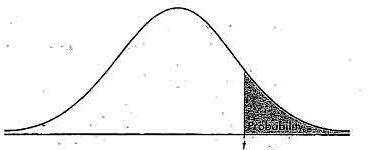
\includegraphics[width=0.8\textwidth]{img/ttest1.jpeg}
			\begin{itemize}
				\item Symmetrical.
				\item \textbf{\color{airforceblue}Significance level}:
				      \begin{itemize}
					      \item E.g., $\text{sig} = 0.05$ or $5\%$ means $M_1$ \& $M_2$ are significantly different for $95\%$ of population.
				      \end{itemize}
				\item Confidence limit: $z = \frac{\text{sig}}{2}$.
			\end{itemize}
		\end{column}
		\begin{column}{0.5\textwidth}
			\centering
			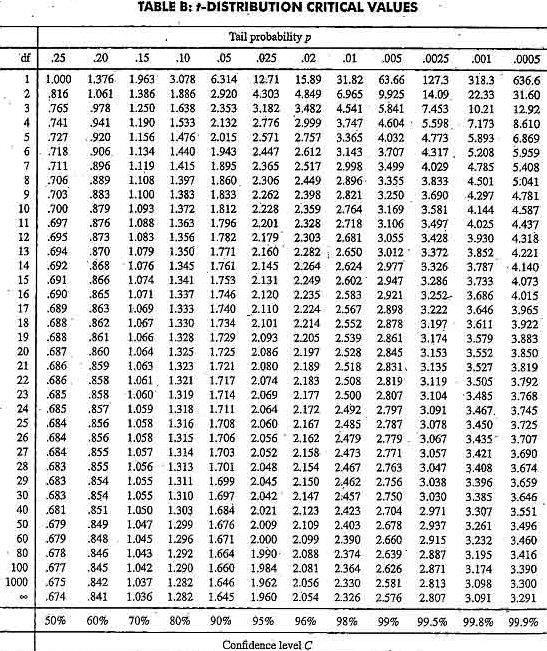
\includegraphics[width=0.7\textwidth]{img/ttest2.jpeg}
		\end{column}
	\end{columns}
\end{frame}

\begin{frame}{Estimating Confidence Intervals: Statistical Significance}
	\textbf{Are $M_1$ and $M_2$ {\color{airforceblue} significantly different}?}
	\begin{itemize}
		\item Compute $t$. Select significance level (E.g., sig = $5 \%$).
		\item Consult table for $t$-distribution:
		      \begin{itemize}
			      \item $t$-distribution is symmetrical:
			            \begin{itemize}
				            \item Typically upper $\%$ points of distribution shown.
			            \end{itemize}
			      \item Find critical value $c$ corresponding to $k-1$ degrees of freedom (here, $9$)
			      \item and for confidence limit $z = \frac{\text{sig}}{2}$ (here, $0.025$).
			      \item $\implies$ Here, critical value $c = 2.262$
		      \end{itemize}
		\item If $t > c$ or $t < -c$, then $t$ value lies in rejection region:
		      \begin{itemize}
			      \item \textbf{Reject null hypothesis} that mean error rates of $M_1$ and $M_2$ are equal.
			      \item Conclude: \textbf{statistically significant difference} between $M_1$ and $M_2$.
		      \end{itemize}
		\item Otherwise, conclude that any difference is chance.
	\end{itemize}
\end{frame}

\begin{frame}{Model Selection: Receiver Operating Characteristics (ROC) Curves}
	\vspace*{-1.5em}
	\begin{columns}
		\begin{column}{0.6\textwidth}
			\begin{itemize}
				\item Visual comparison of classification models.
				\item Compares and shows \textit{trade-off} between TPR and FPR:
				      \begin{itemize}
					      \item True Positive Rate (\textbf{TPR}): Proportion of positive tuples correctly classified as positive.\\
					            $\rightarrow$ sensitivity or recall $= \frac{\text{TP}}{\text{P}}$
					      \item False Positive Rate (\textbf{FPR}:) Proportion of negative tuples correctly classified as negative.\\
					            $\rightarrow \text{FPR} = \frac{\text{FP}}{\text{N}} = 1 - \text{Specificity}$
				      \end{itemize}

				\item \textbf{The area under the ROC curve is a
						      {\color{airforceblue}measure of the accuracy} of the model.}
				      Maximum area of $1.0$ for a perfect classifier.
				\item \textbf{The closer to the diagonal line (i.e. the closer the
					      area is to $0.5$), the less accurate is the model.}

			\end{itemize}
		\end{column}
		\begin{column}{0.4\textwidth}
			\vspace*{-1.5em}
			\begin{figure}
				\centering
				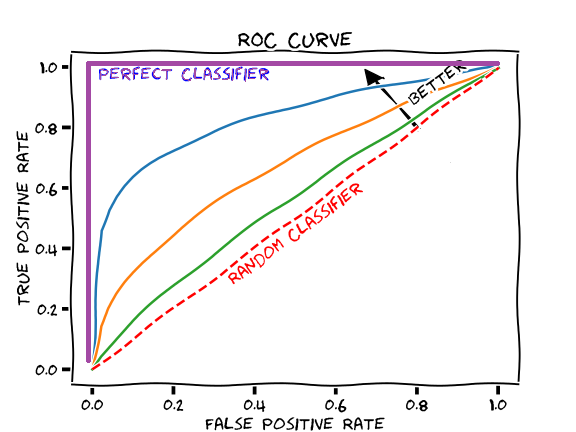
\includegraphics[width=\textwidth]{img/roc-curve.png}
			\end{figure}
			\vspace*{-0.5em}
			\scriptsize
			How to draw: Order tuples in decreasing order of probability.
			\begin{itemize}
				\item If TP move up TPR and plot point.
				\item If negative tuple classified as positive: move both FPR and FPR.
			\end{itemize}
		\end{column}
	\end{columns}
\end{frame}

\begin{frame}{Other Aspects of Model Selection}
	\begin{itemize}
		\item \textbf{Speed}
		      \begin{itemize}
			      \item Computational cost to train a classifier.
			      \item Time to use model (prediction time).
		      \end{itemize}
		\item \textbf{Robustness}, i. e. the ability to make accurate predictions.
		      \begin{itemize}
			      \item Noisy data.
			      \item Missing values.
		      \end{itemize}
		\item \textbf{Scalability}, i . e. efficient construction of classifiers on an abundant amount of training tuples.
		\item \textbf{Interpretability}, refers to understanding and insight
		      \begin{itemize}
			      \item Typically subjective and difficult to access.
			      \item Decision trees and classification rules are easy to interpret, but interpretability degrades with the size.
		      \end{itemize}
		\item \textit{Other measures} such as goodness of rules, decision-tree size or compactness of classification rules.
	\end{itemize}
\end{frame}
